% --------------------------------------------------------------
% This is all preamble stuff that you don't have to worry about.
% Head down to where it says "Start here"
% --------------------------------------------------------------
 
\documentclass[12pt]{article}

\usepackage[margin=1in]{geometry} 
\usepackage{amsmath,amsthm,amssymb}
\usepackage[margin=1in]{geometry} 
\usepackage{amsmath,amsthm,amssymb}
%\numberwith{equation}{section}
%\usepackage[spanish]{babel} %Castellanización
\usepackage[T1]{fontenc} %escribe lo del teclado
\usepackage{inputenc} %Reconoce algunos símbolos
\usepackage{lmodern} %optimiza algunas fuentes
\usepackage{graphicx}
\graphicspath{ {images/} }
\usepackage{hyperref} % Uso de links

% To Display Chinese words
\usepackage{xeCJK}
% To Display Code
% \usepackage{listings}
\usepackage{minted}
% To Display csv file
\usepackage{csvsimple}
 
\newcommand{\N}{\mathbb{N}}
\newcommand{\Z}{\mathbb{Z}}
 
\newenvironment{theorem}[2][Theorem]{\begin{trivlist}
\item[\hskip \labelsep {\bfseries #1}\hskip \labelsep {\bfseries #2.}]}{\end{trivlist}}
\newenvironment{lemma}[2][Lemma]{\begin{trivlist}
\item[\hskip \labelsep {\bfseries #1}\hskip \labelsep {\bfseries #2.}]}{\end{trivlist}}
\newenvironment{exercise}[2][Exercise]{\begin{trivlist}
\item[\hskip \labelsep {\bfseries #1}\hskip \labelsep {\bfseries #2.}]}{\end{trivlist}}
\newenvironment{problem}[2][Problem]{\begin{trivlist}
\item[\hskip \labelsep {\bfseries #1}\hskip \labelsep {\bfseries #2.}]}{\end{trivlist}}
\newenvironment{question}[2][Question]{\begin{trivlist}
\item[\hskip \labelsep {\bfseries #1}\hskip \labelsep {\bfseries #2.}]}{\end{trivlist}}
\newenvironment{corollary}[2][Corollary]{\begin{trivlist}
\item[\hskip \labelsep {\bfseries #1}\hskip \labelsep {\bfseries #2.}]}{\end{trivlist}}

\newenvironment{solution}{\begin{proof}[Solution]}{\end{proof}}
 
\begin{document}
 
% --------------------------------------------------------------
%                         Start here
% --------------------------------------------------------------
 
\title{2019 Deep Learning and Practice \\ Lab 2 : EEG classification}
\author{0756110 李東霖}

\maketitle
\section{Introduction}

In this experiment, I implemented EEGNet and DeepConvNet with three activation functions including ReLU, Leaky ReLU and ELU to classify signals of brain into two classes.
\par \ \par
 The objectives of the experiment are as follows:

\begin{itemize}
\item To show the highest accuracy of two models with three activation functions.
\item To visualize the accuracy trend.
\end{itemize}

\subsection{Dataset}

This dataset has two channel of 750 data points each. The label of two classes in dataset are left-handed and right-handed.

\begin{figure}
\centering
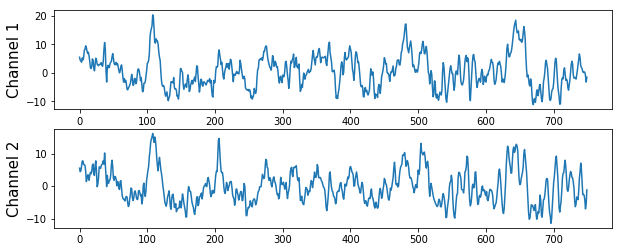
\includegraphics[scale=0.65]{Images/EEGData.png} 
\caption{2 bipolar EEG signals}
\end{figure}

\section{Experiment setup}

\subsection{Convert Data to Tensor}

To leverage \verb|DataLoader| from  \verb|pytorch|, I convert  \verb|numpy| array to  \verb|TensorDataset| and make  \verb|TensorDataset| as  \verb|DataLoader|, So I can easily train my model with specific batch size.

\begin{minted}[frame=lines]{python}
import dataloader
import torch
from torch.utils.data import TensorDataset, DataLoader

def gen_dataset(train_x, train_y, test_x, test_y):
    datasets = []
    for x, y in [(train_x, train_y), (test_x, test_y)]:
        x = torch.stack(
            [torch.Tensor(x[i]) for i in range(x.shape[0])]
        )
        y = torch.stack(
            [torch.Tensor(y[i:i+1]) for i in range(y.shape[0])]
        )
        datasets += [TensorDataset(x, y)]
        
    return datasets

train_dataset, test_dataset = gen_dataset(*dataloader.read_bci_data())
train_loader = DataLoader(train_dataset, batch_size=batch_size)
test_loader = DataLoader(test_dataset, len(test_dataset))
\end{minted}

\subsection{EEGNet}

Reference from EEGNet: A Compact Convolutional Neural Network for EEG-based Brain-Computer Interfaces. 

\begin{figure}[H]
\centering
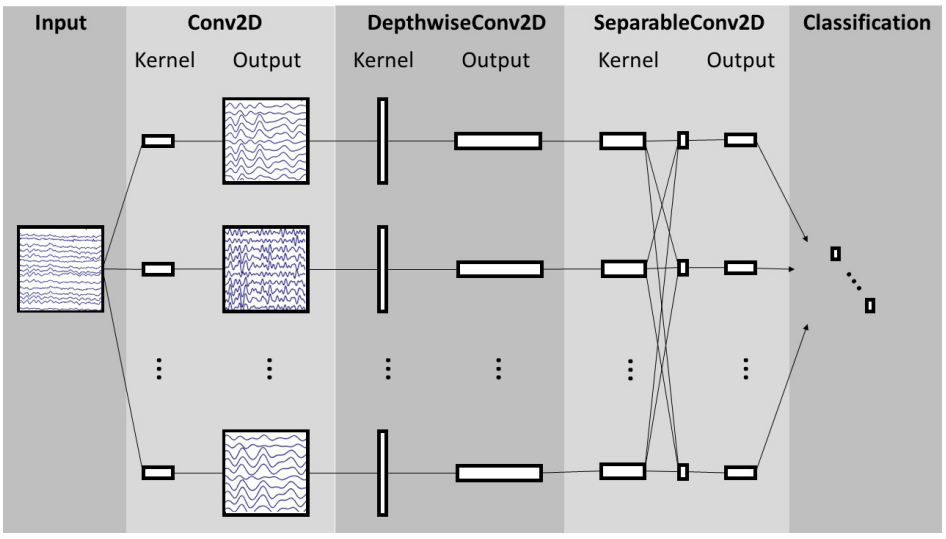
\includegraphics[width=\linewidth]{Images/OverallEEGNet.png}
\caption{Overall visualization of the EEGNet architecture}
\end{figure}

The first Conv2D learns how to extract features from signals, then DepthwiseConv2D learns how to combine multiple channel signal into one for each input. The DepthwiseConv2D is different from normal convolution layers in it doesn't  fully connect between input and output. Finally SeparableConv2D learns how to extract features from output of DepthwiseConv2D.

\begin{minted}[frame=lines]{python}
class EEGNet(nn.Module):
    def __init__(self, activation=None, dropout=0.25):
        super(EEGNet, self).__init__()
        
        if not activation:
            activation = nn.ELU
        
        self.firstconv = nn.Sequential(
            nn.Conv2d(
                1, 16, kernel_size=(1, 51),
                stride=(1,1), padding=(0,25), bias=False
            ),
            nn.BatchNorm2d(16)
        )
        self.depthwiseConv = nn.Sequential(
            nn.Conv2d(
                16, 32, kernel_size=(2,1),
                stride=(1,1), groups=16, bias=False
            ),
            nn.BatchNorm2d(32),
            activation(),
            nn.AvgPool2d(kernel_size=(1, 4), stride=(1, 4), padding=0),
            nn.Dropout(p=dropout)
        )
        self.separableConv = nn.Sequential(
            nn.Conv2d(
                32, 32, kernel_size=(1, 15), 
                stride=(1,1), padding=(0, 7), bias=False
            ),
            nn.BatchNorm2d(32),
            activation(),
            nn.AvgPool2d(kernel_size=(1, 8), stride=(1, 8), padding=0),
            nn.Dropout(p=dropout)
        )
        self.classify = nn.Sequential(
            nn.Linear(736, 2, bias=True)
        )
        
    def forward(self, x):
        x = self.firstconv(x)
        x = self.depthwiseConv(x)
        x = self.separableConv(x)
        # flatten
        x = x.view(-1, self.classify[0].in_features)
        x = self.classify(x)
        return x
\end{minted}

\subsection{DeepConvNet}

This model architecture has multiple convolution layers. Just like normal CNN. It is comparison to EEGNet in the paper.
\par \ \par
To easily modify number of layers and number of kernels, I use one array to present how to build DeepConvNet. e.g. [25, 50] means first layer has 25 output channels and second layer has 50 output channels.

\begin{minted}[frame=lines]{python}
from functools import reduce
class DeepConvNet(nn.Module):
    def __init__(self, activation=None, deepconv=[25,50,100,200], dropout=0.5):
        super(DeepConvNet, self).__init__()
        
        if not activation:
            activation = nn.ELU
        
        self.deepconv = deepconv
        self.conv0 = nn.Sequential(
            nn.Conv2d(
                1, deepconv[0], kernel_size=(1, 5),
                stride=(1,1), padding=(0,0), bias=True
            ),
            nn.Conv2d(
                deepconv[0], deepconv[0], kernel_size=(2,1),
                stride=(1,1), padding=(0,0), bias=True
            ),
            nn.BatchNorm2d(deepconv[0]),
            activation(),
            nn.MaxPool2d(kernel_size=(1,2)),
            nn.Dropout(p=dropout)
        )
        
        for idx in range(1, len(deepconv)):
            setattr(self, 'conv'+str(idx), nn.Sequential(
                nn.Conv2d(
                    deepconv[idx-1], deepconv[idx], kernel_size=(1,5),
                    stride=(1,1), padding=(0,0), bias=True
                ),
                nn.BatchNorm2d(deepconv[idx]),
                activation(),
                nn.MaxPool2d(kernel_size=(1, 2)),
                nn.Dropout(p=dropout)
            ))
        
        
        flatten_size =  deepconv[-1] * reduce(
            lambda x,_: round((x-4)/2), deepconv, 750)
        self.classify = nn.Sequential(
            nn.Linear(flatten_size, 2, bias=True),
        )
    
    def forward(self, x):
        for i in range(len(self.deepconv)):
            x = getattr(self, 'conv'+str(i))(x)
        # flatten
        x = x.view(-1, self.classify[0].in_features)
        x = self.classify(x)
        return x
\end{minted}

\subsection{Activation functions}

Use three kinds of activation functions and compare their outputs.

\begin{itemize}
\item ReLU
\end{itemize}

\begin{equation}
ReLU(x) = max(0, x)
\end{equation}
\begin{itemize}
\item Leaky ReLU
\end{itemize}

\begin{equation}
LeakyReLU(x) = \left\{\begin{array}{ll}
x, & \text{if  x > 0} \\
\text{negative\_slope} \times x, & \text{otherwise}
\end{array}\right.
\end{equation}

\begin{itemize}
\item ELU
\end{itemize}

\begin{equation}
ELU(x) = max(0, x) + min(0, \alpha \ast (exp(x) - 1) )
\end{equation}

\begin{figure}[H]
\centering
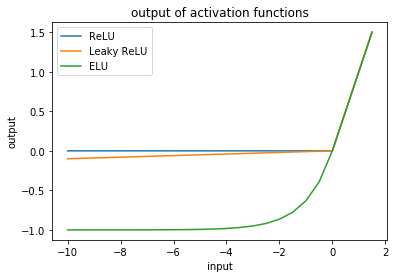
\includegraphics{Images/OutputActivation.png}
\caption{output of activation functions}
\end{figure}

The big difference between them is output from negative input value. It also means different gradient from negative input value. Let take look at gradient output. To see their difference.

\begin{figure}[H]
\centering
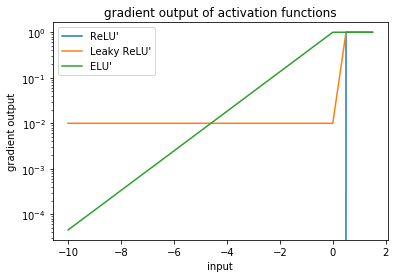
\includegraphics{Images/GradientOutputActivation.png}
\caption{gradient output of activation functions}
\end{figure}

The ReLU always get zero gradient (log axis can't show zero value) from negative input value that will cause vanishing gradient problem. To avoid vanishing gradient problem, the Leaky ReLU and ELU design different equation at negative input value. In addition, computing volumes of ELU is bigger than Leaky ReLU. 

\section{Experimental results}

Common hyper parameters : 
\begin{itemize}
\item optimizer : Adam
\item criterion (loss) : CrossEntropy
\item epoch size : 300
\item batch size : 64
\item learning rate for EEGNet : 0.01
\item learning rate for DeepConvNet : 0.001
\end{itemize}

\subsection{The highest testing accuracy}

\csvautotabular{AccuracyResult.csv}

\subsection{Comparison figures}

\begin{figure}[H]
\centering
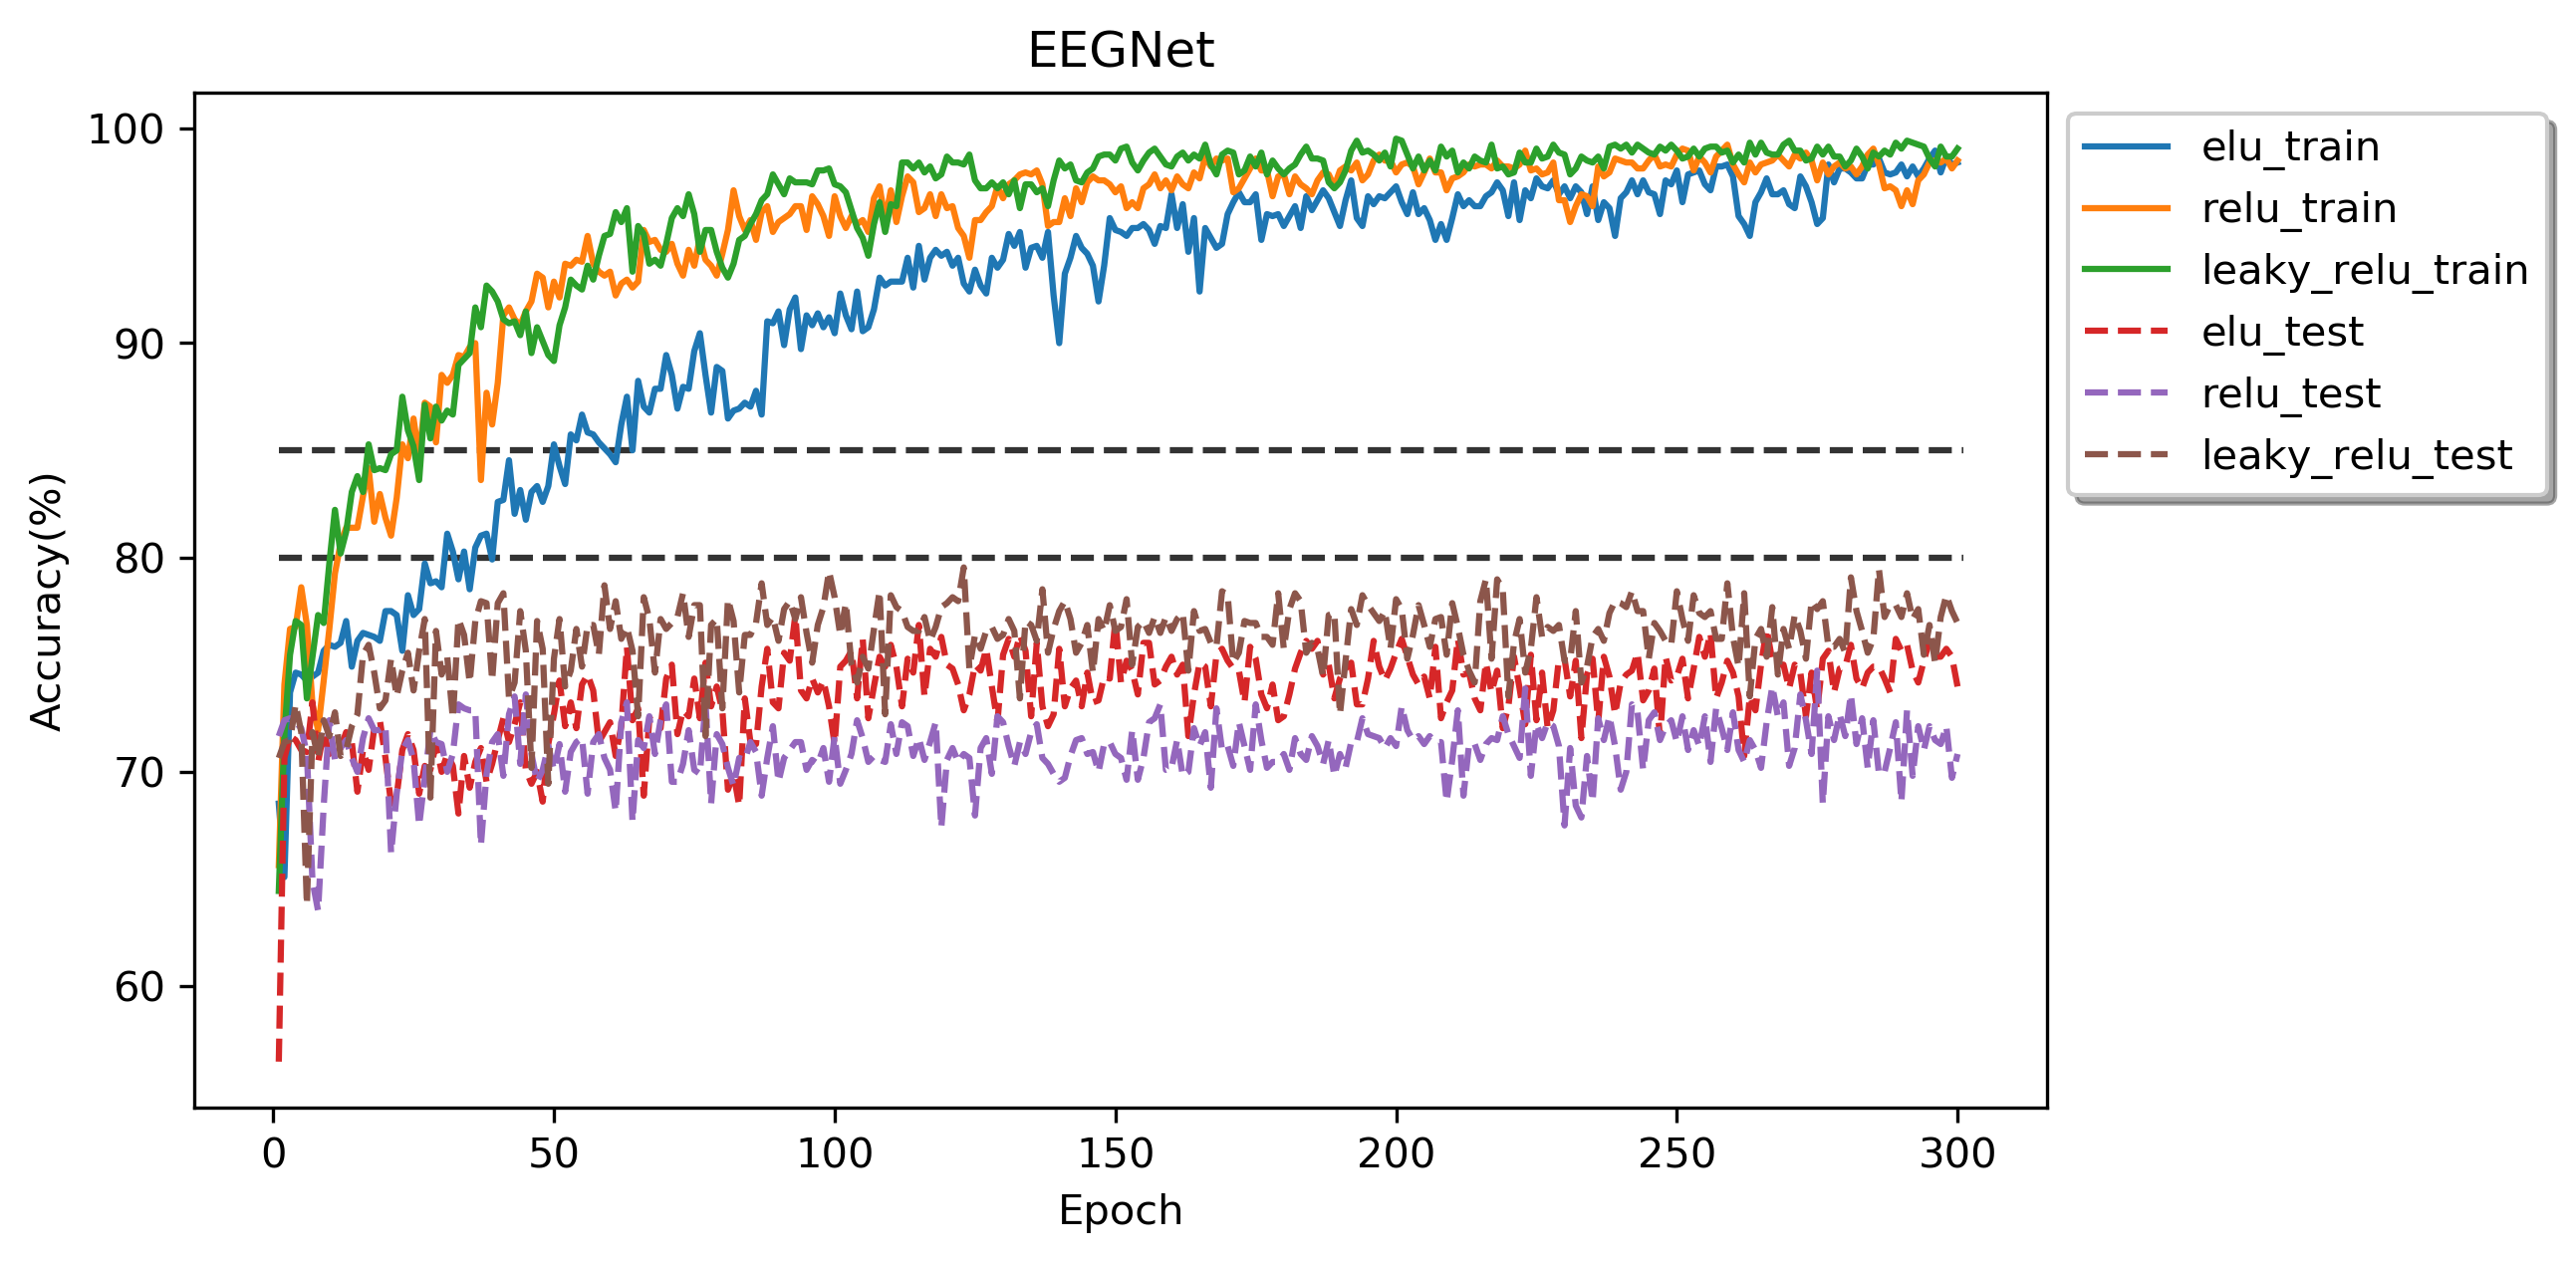
\includegraphics[width=\linewidth]{Images/EEGNet.png}
\caption{Default EEGNet}
\end{figure}

\begin{figure}[H]
\centering
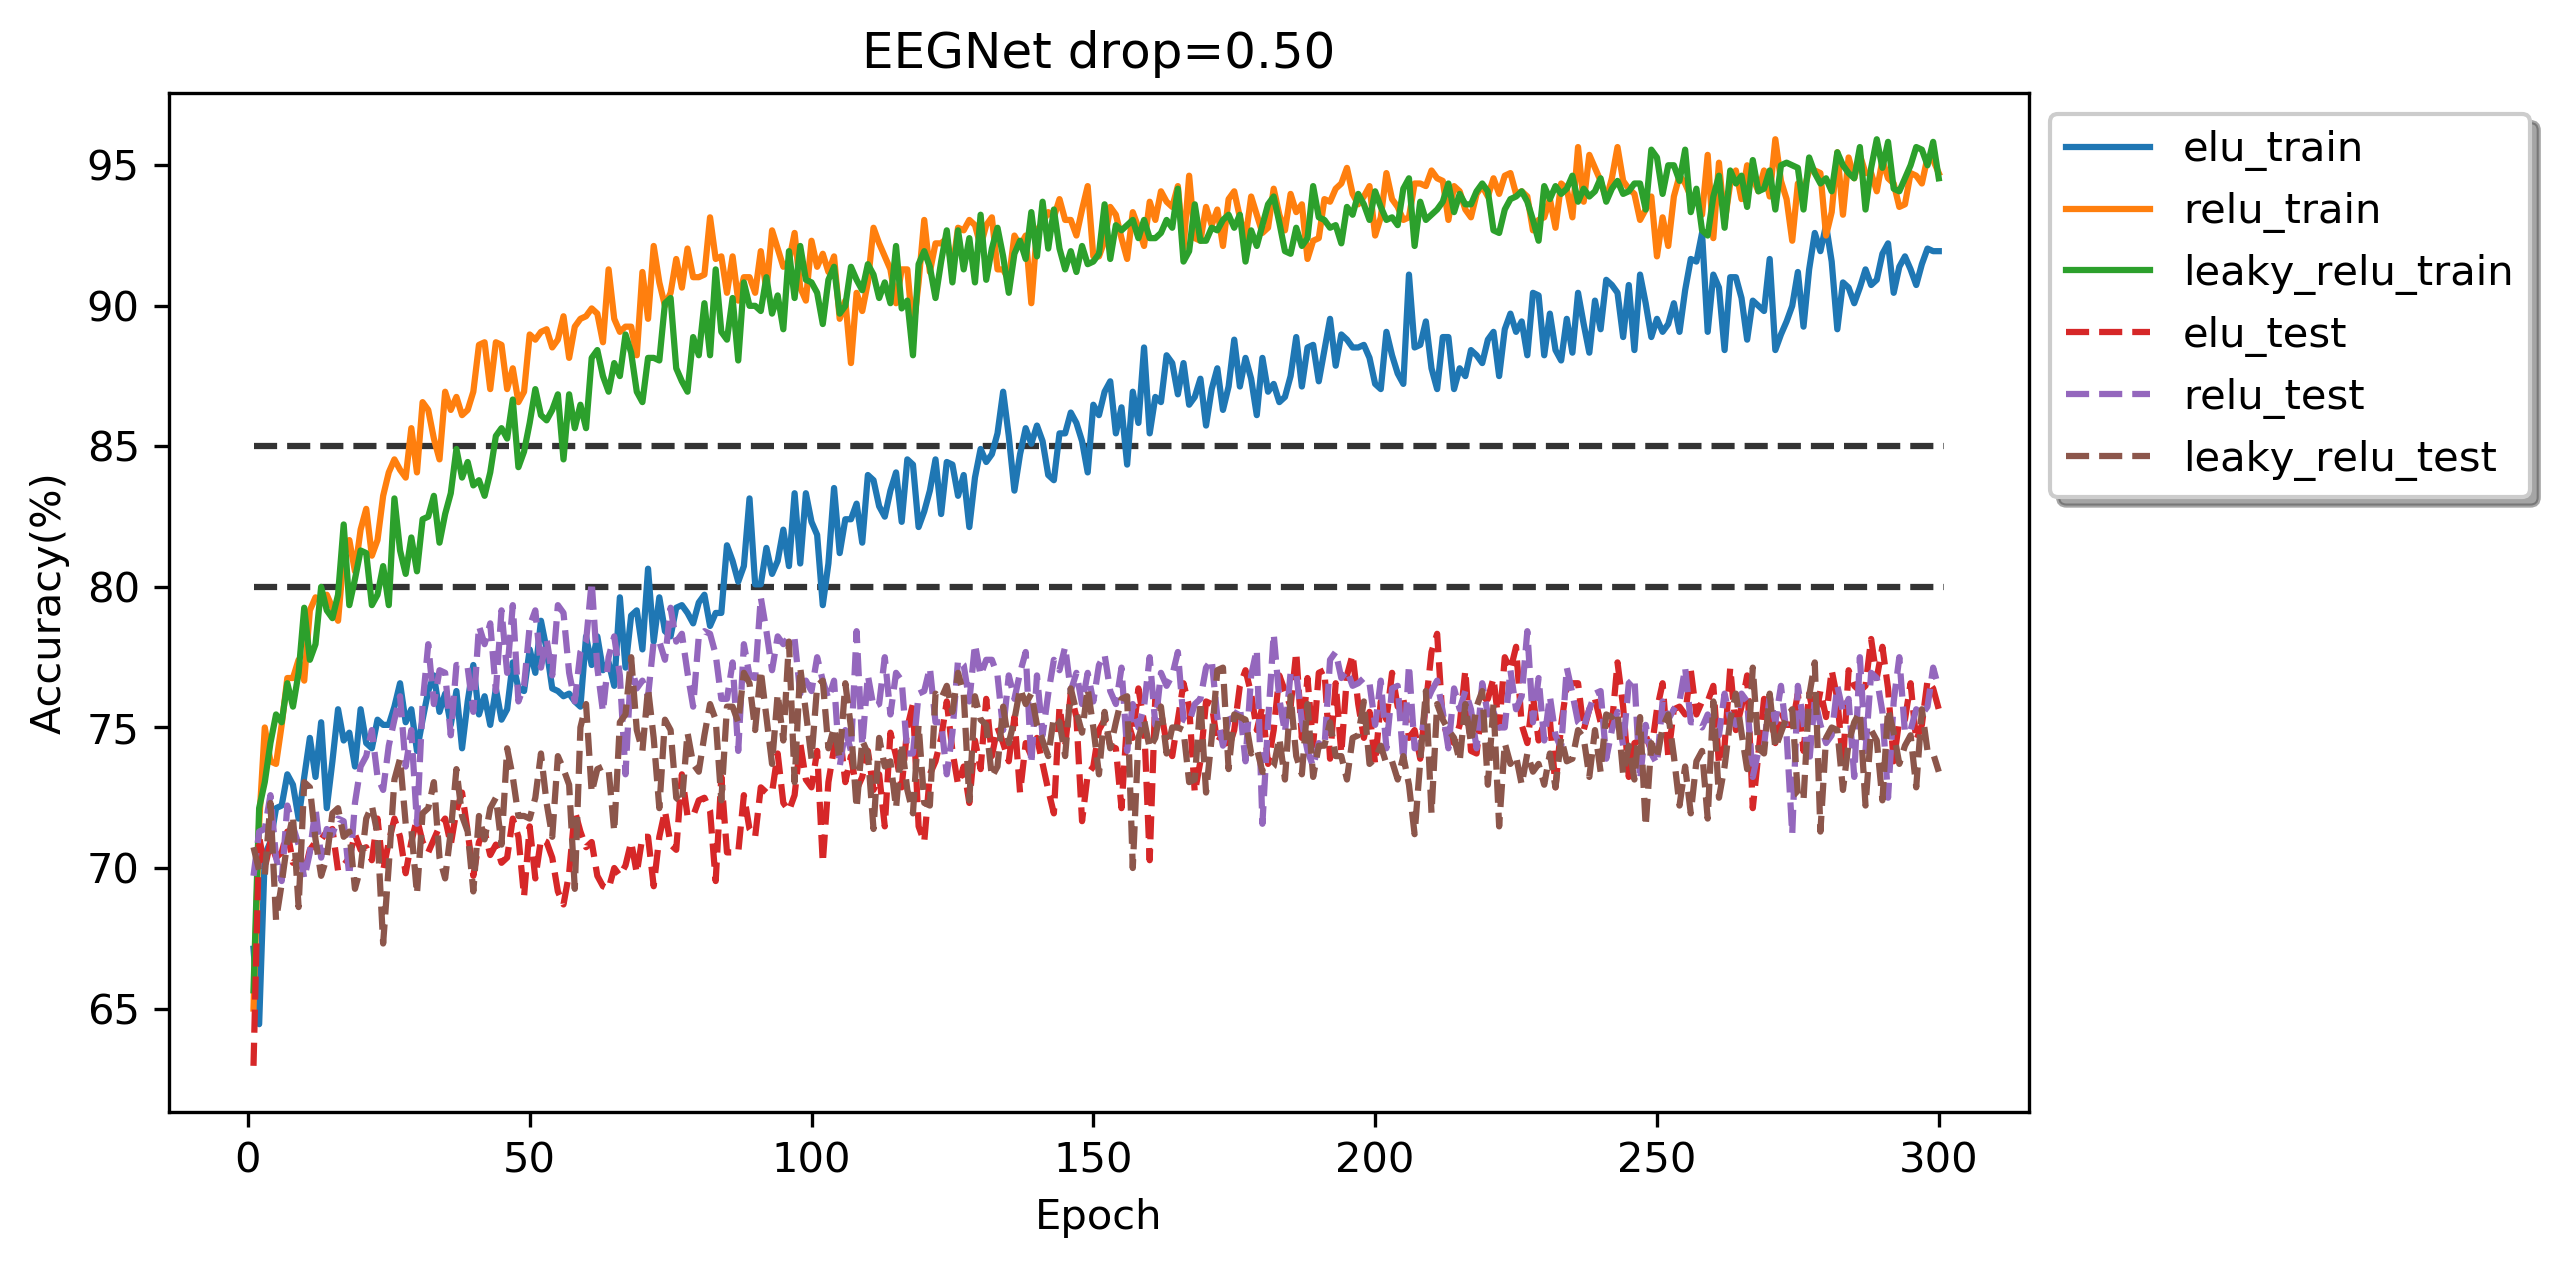
\includegraphics[width=\linewidth]{Images/EEGNet_drop=050.png}
\caption{Modified EEGNet dropout = 0.5}
\end{figure}

\begin{figure}[H]
\centering
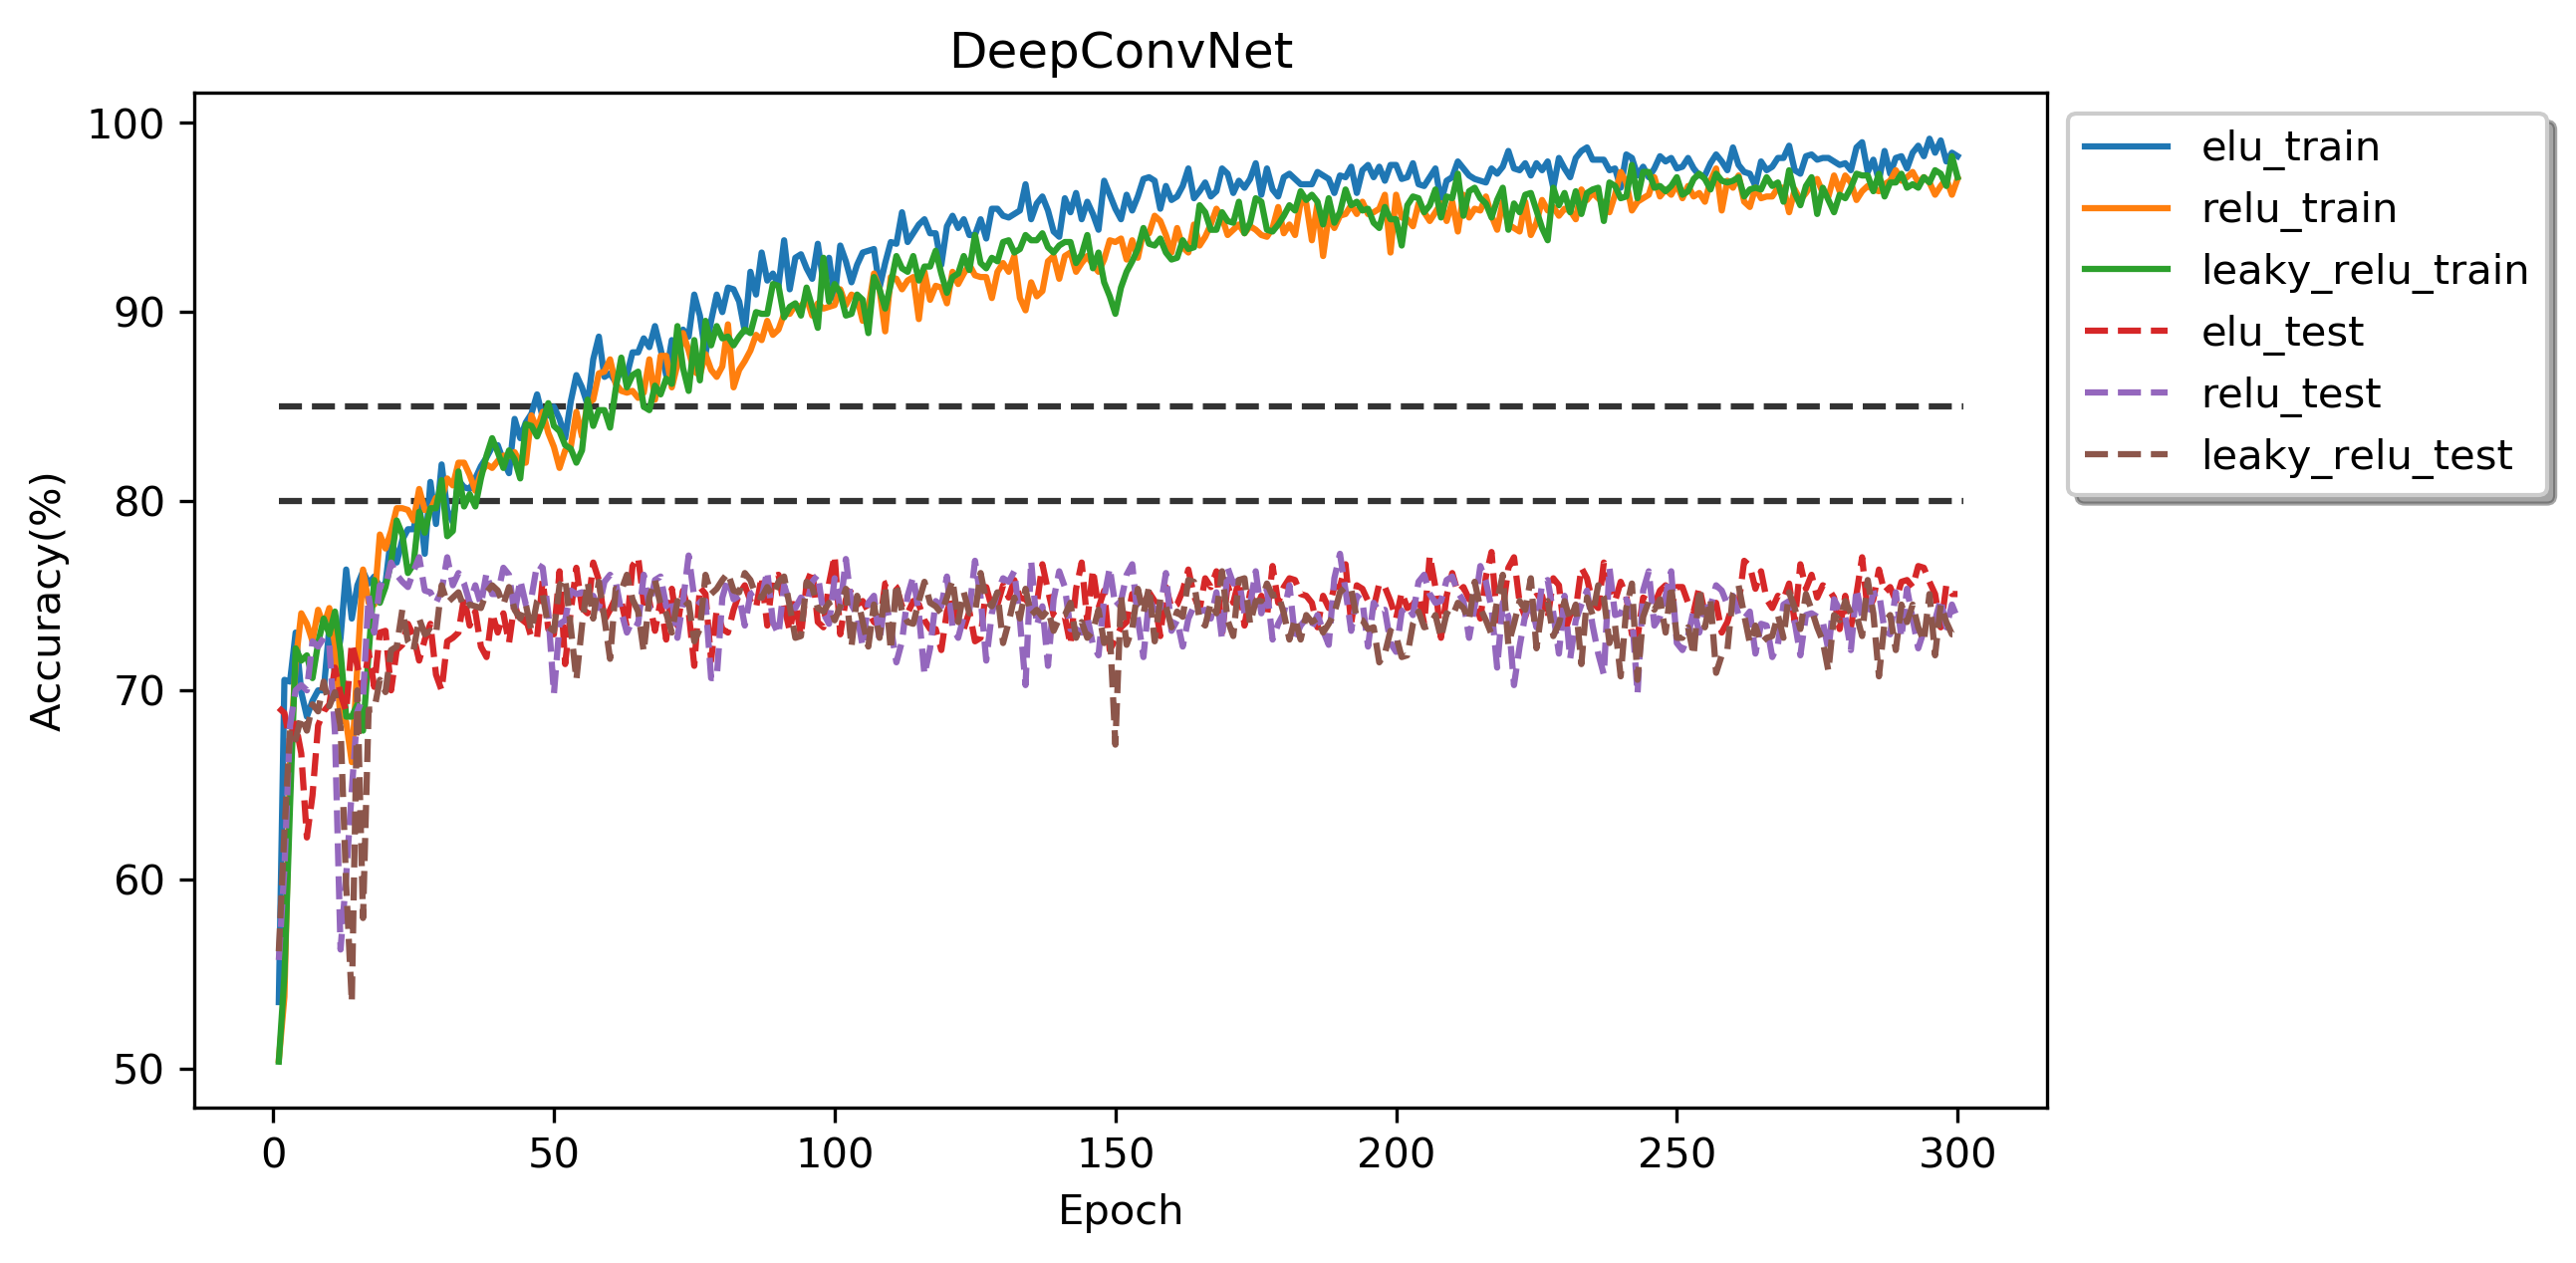
\includegraphics[width=\linewidth]{Images/DeepConvNet.png}
\caption{Default DeepConvNet}
\end{figure}

\begin{figure}[H]
\centering
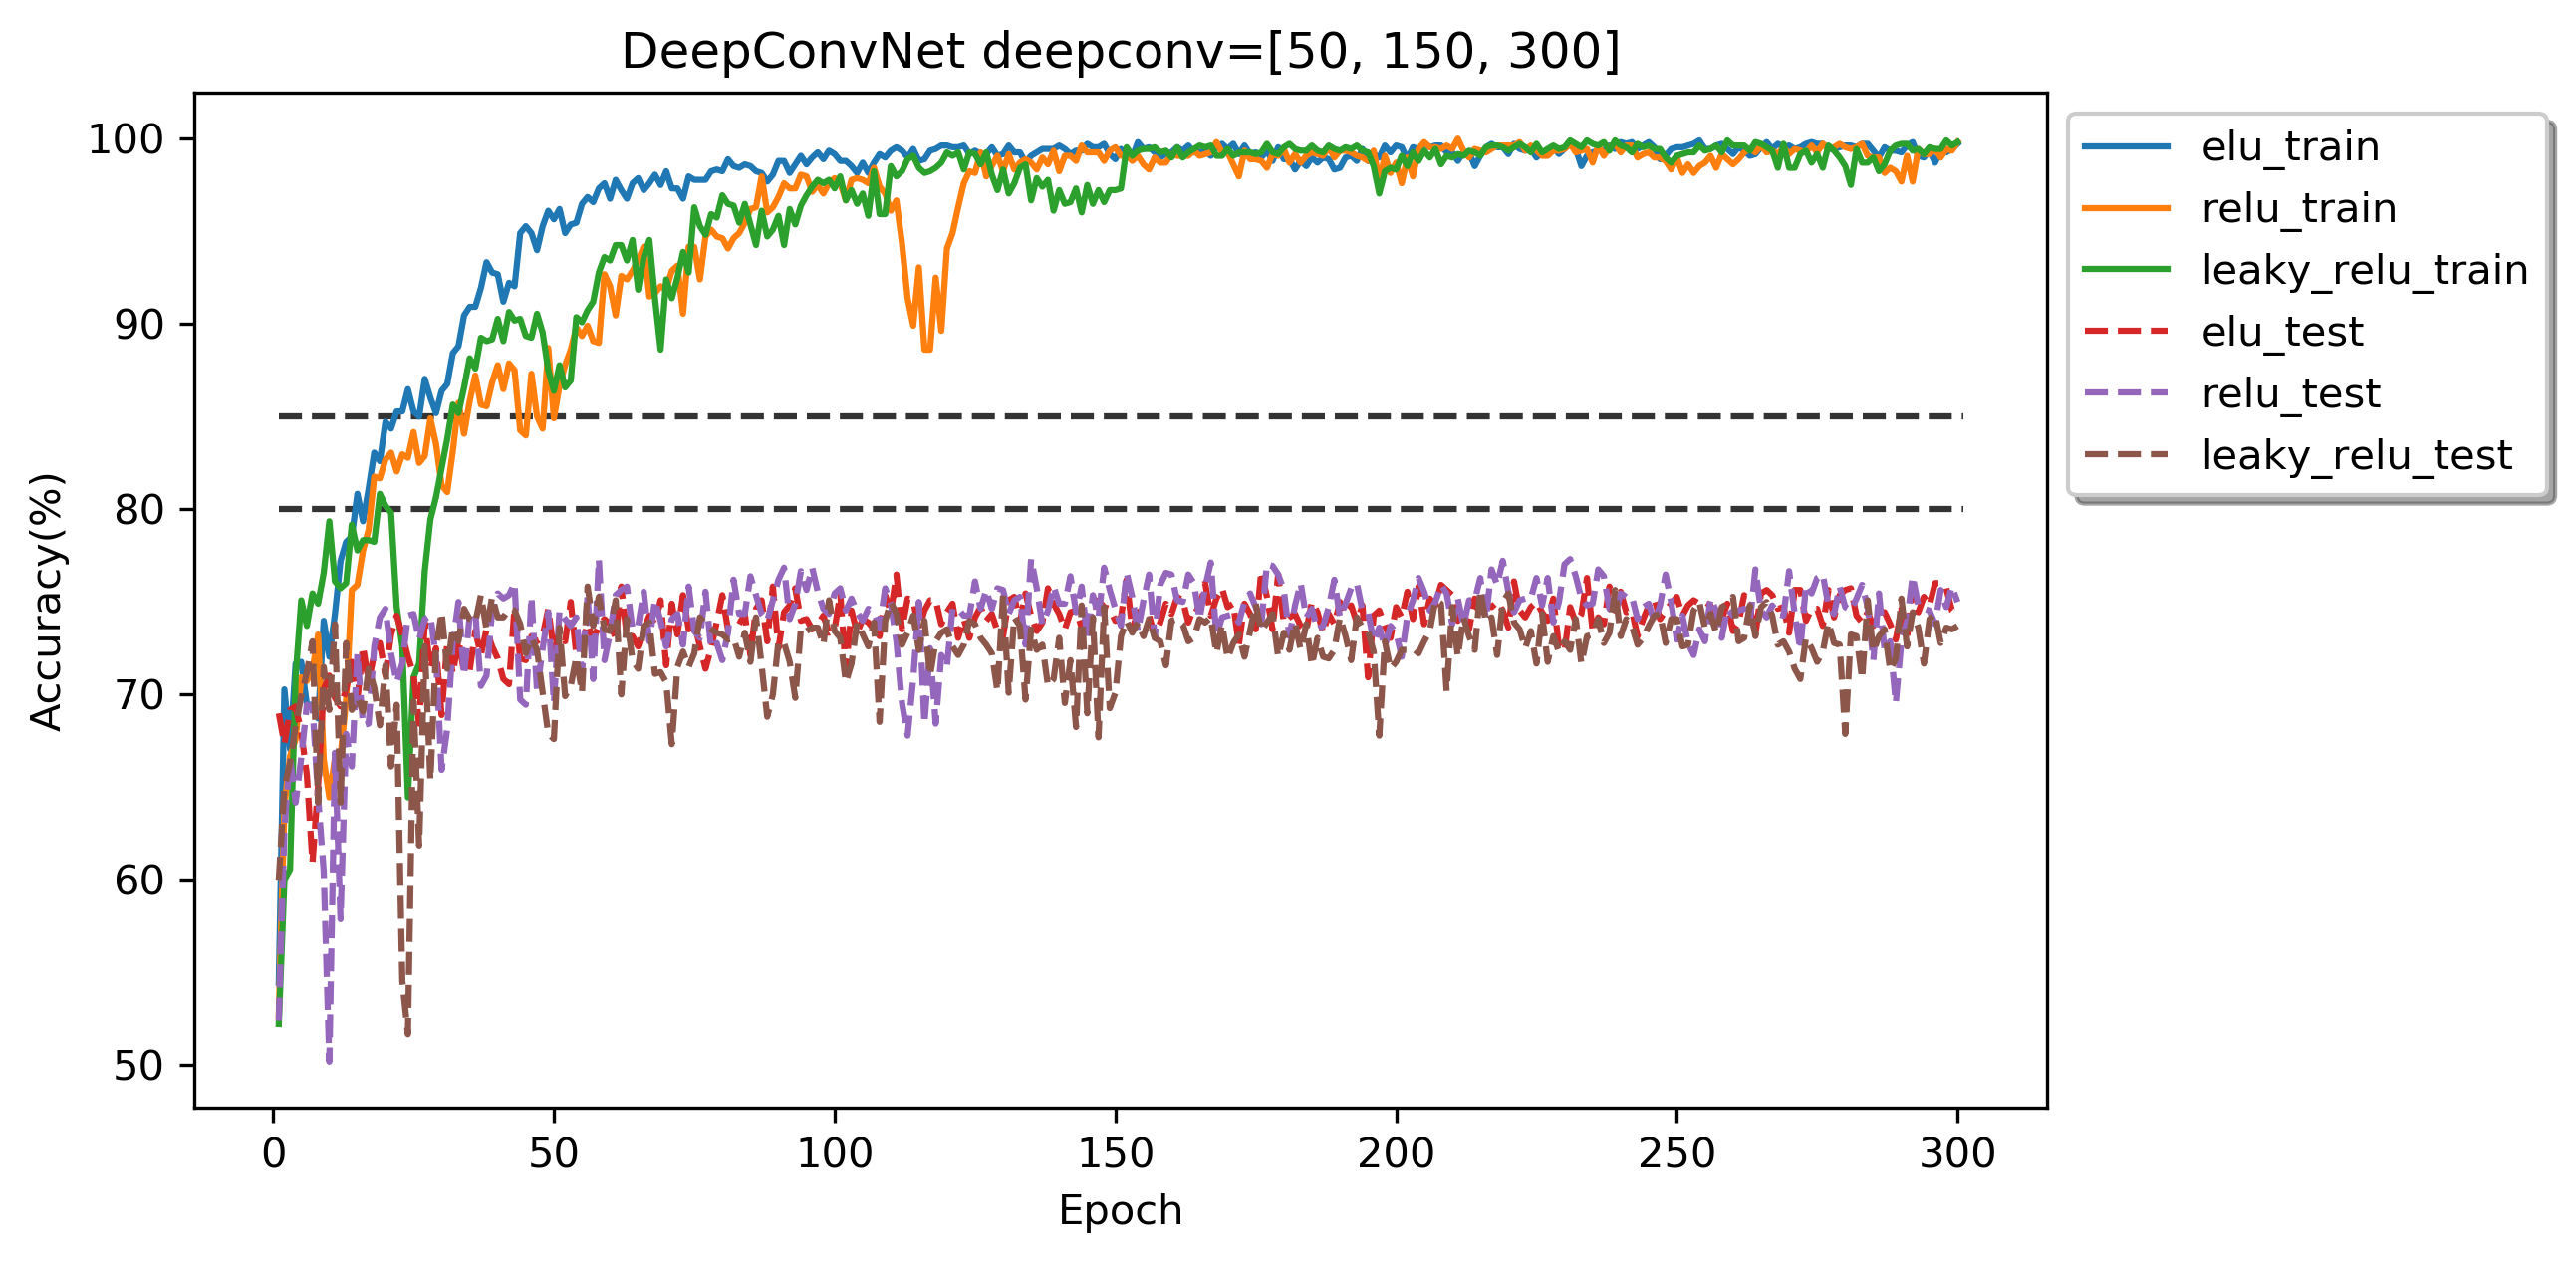
\includegraphics[width=\linewidth]{Images/DeepConvNet_deepconv=[50,150,300].png}
\caption{Modified DeepConvNet layers = [50, 150, 300]}
\end{figure}

\section{Discussion}

\subsection{Dropout and BatchNorm layers with evaluation mode}

Because of dropout layer, outputs of model aren't always the same. To solve this problem and leverage all features from testing dataset and that increase accuracy, I set model as evaluation mode when testing. The dropout layer doesn't drop any input value when model is evaluation mode.

\begin{figure}[H]
\centering
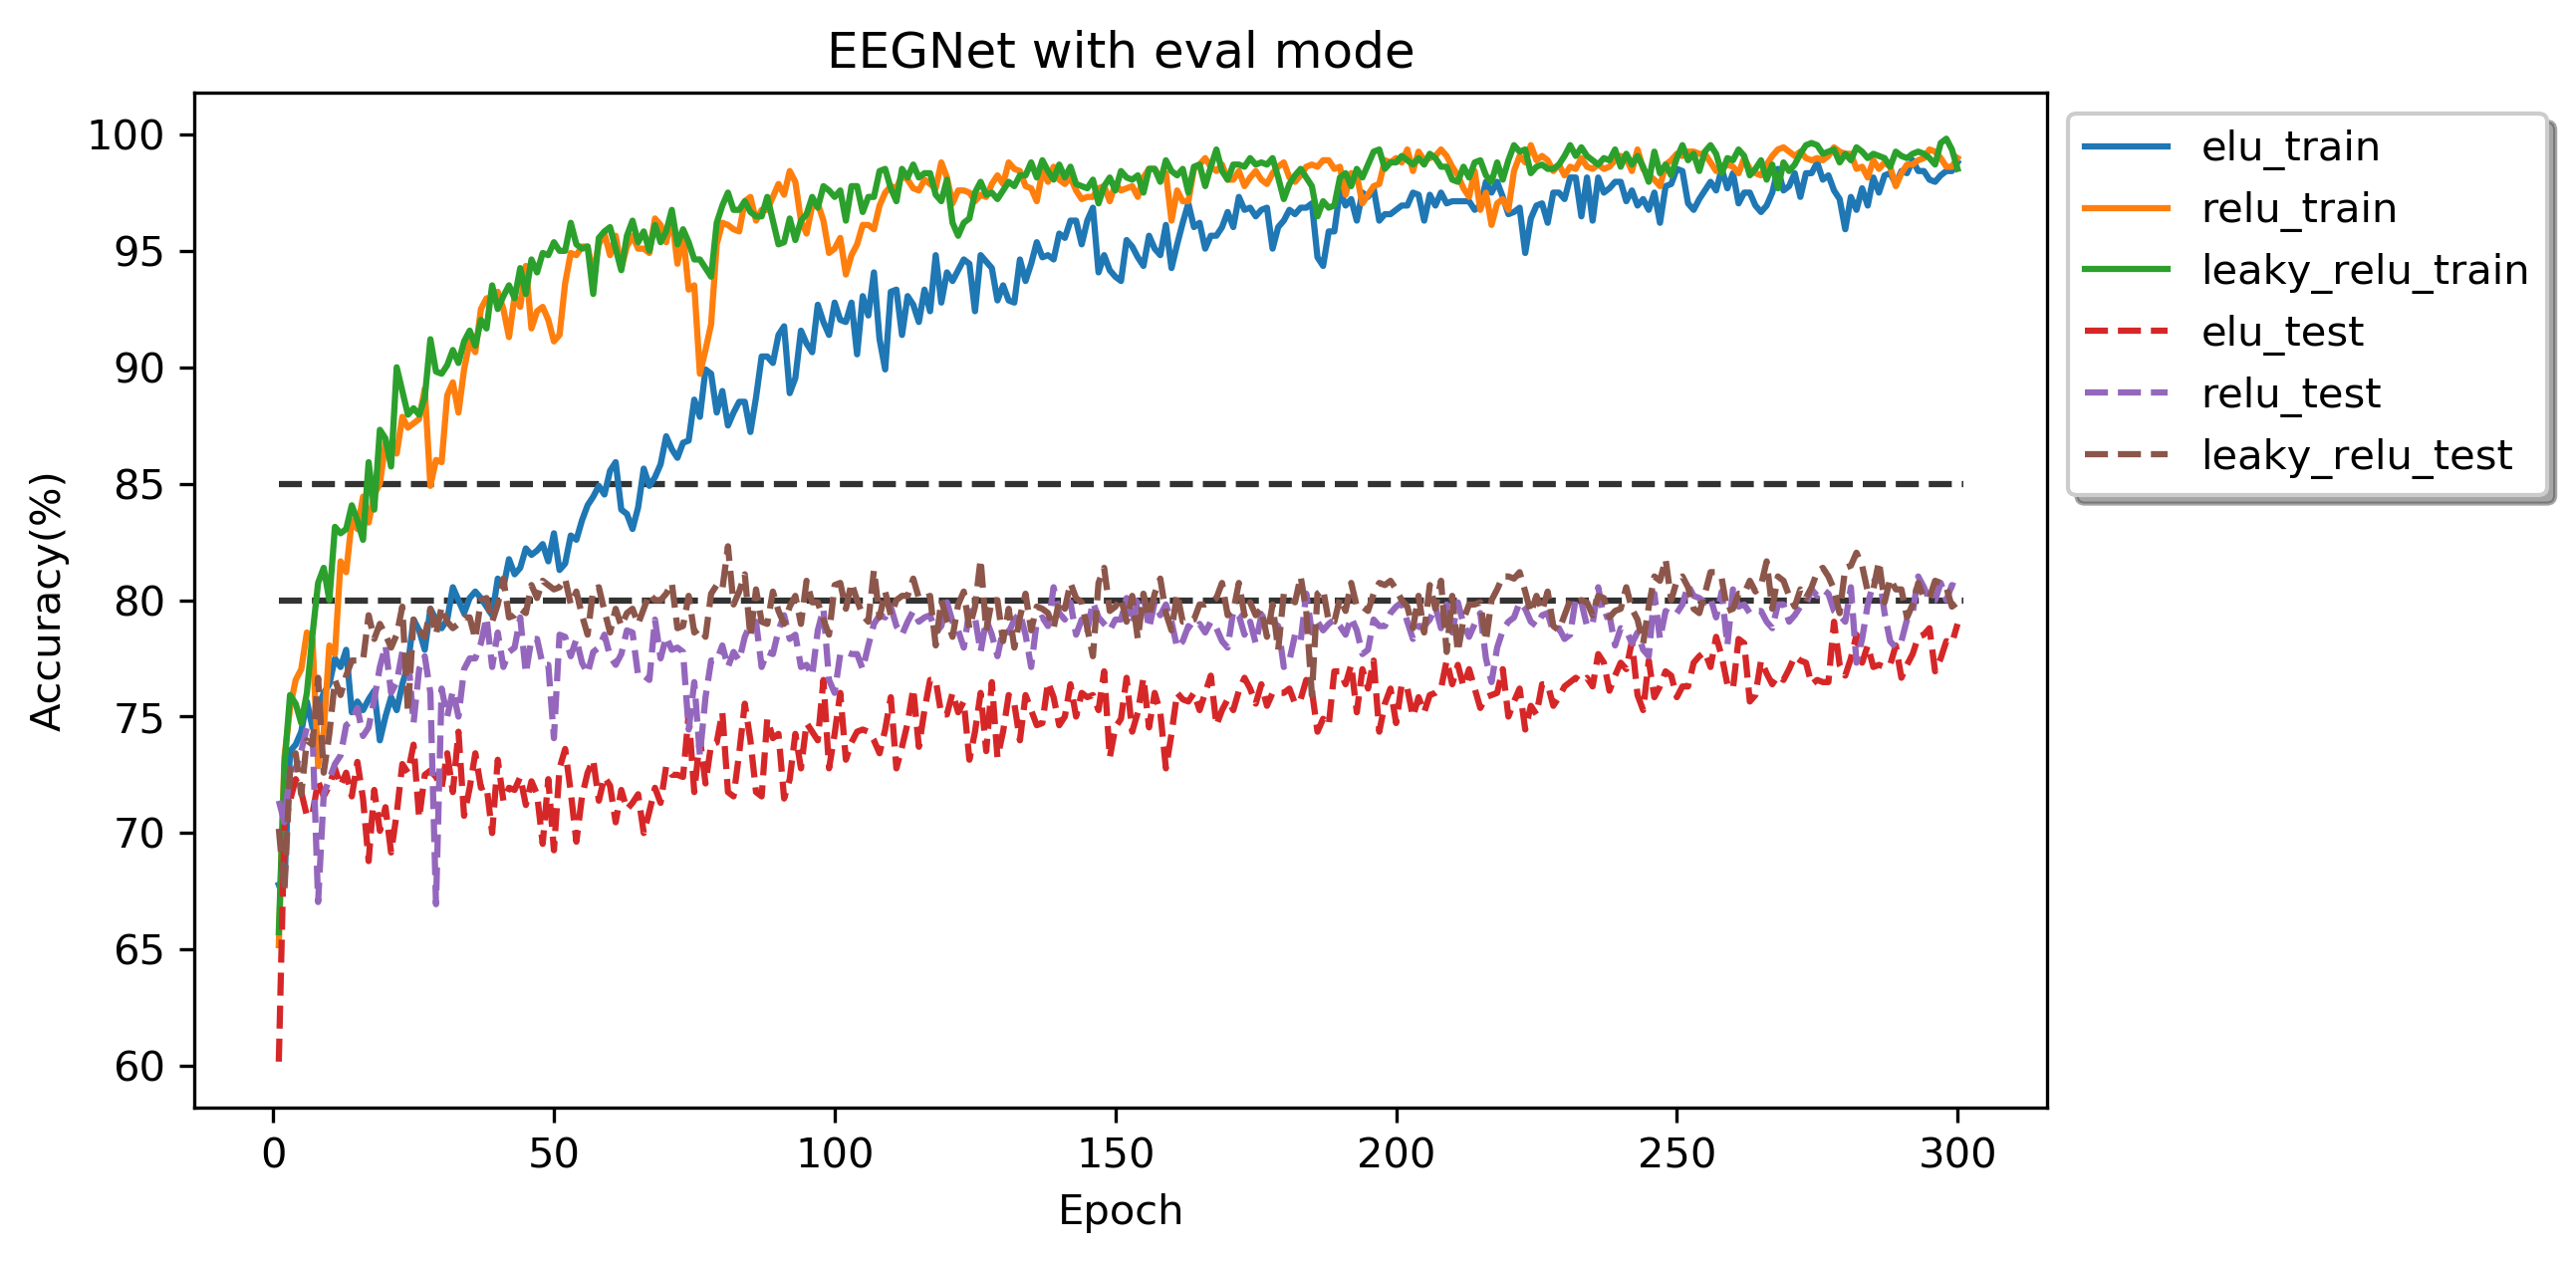
\includegraphics[width=\linewidth]{Images/EEGNetWithEvalMode.png}
\caption{EEGNet with evaluation mode}
\end{figure}

Then you can find the testing accuracy are more stable than model without evaluation mode.
\par \ \par
The evaluation mode also impact BatchNorm layer. BatchNorm layer estimate mean and variance from input values. And evaluation mode can avoid the layer estimating testing input.

\subsection{Dropout influence}

The dropout layer is used in both models.  Hyper parameter of dropout layer is  dropout rate that decide how many chance input value becomes zero. If dropout rate is bigger, more input values will become zero, vice versa. The dropout layer causes unstable in output accuracy of model but it can solve overfitting problem. Because model can't learn all feature from training data when training (some input become zero). That means a pattern exist in data even if some features are dropped out, and model need to learn that pattern.
\par \ \par
To observe the influence from dropout rate, I tried to modify dropout rate in both models and shown the 
result as follows.

\newpage

\begin{itemize}
\item dropout rate = 0.9

\begin{figure}[H]
\centering
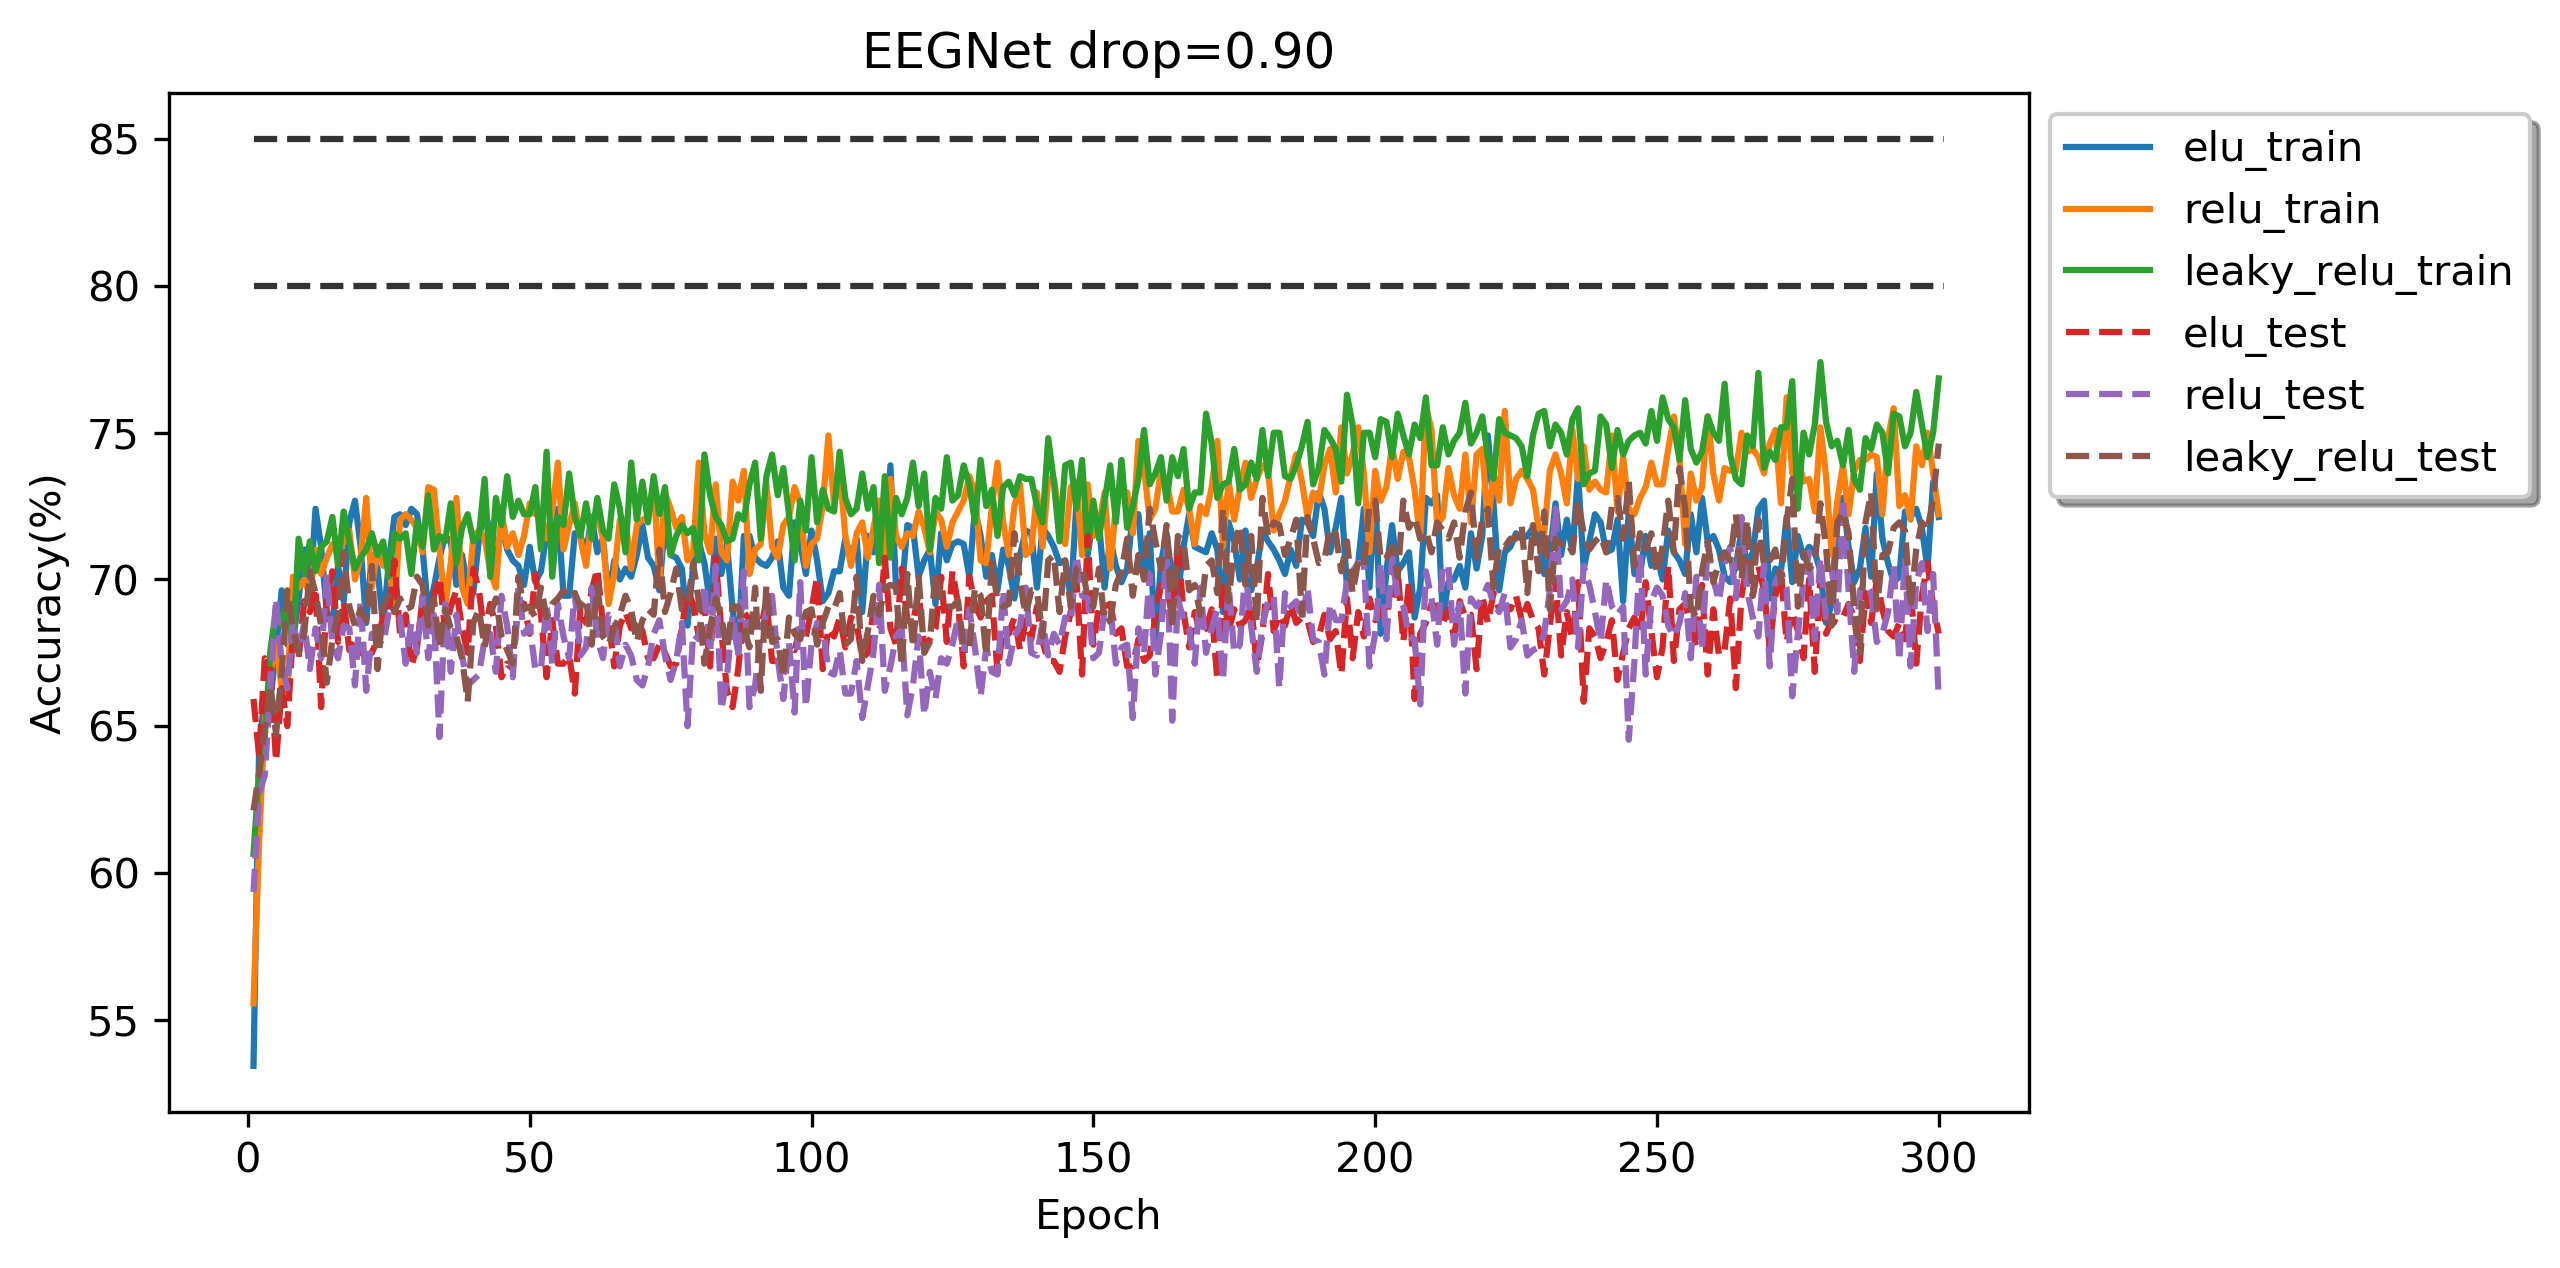
\includegraphics[width=\linewidth]{Images/EEGNetdrop=090.png}
\caption{EEGNet dropout rate = 0.9}
\end{figure}

\item dropout rate = 0.5

\begin{figure}[H]
\centering
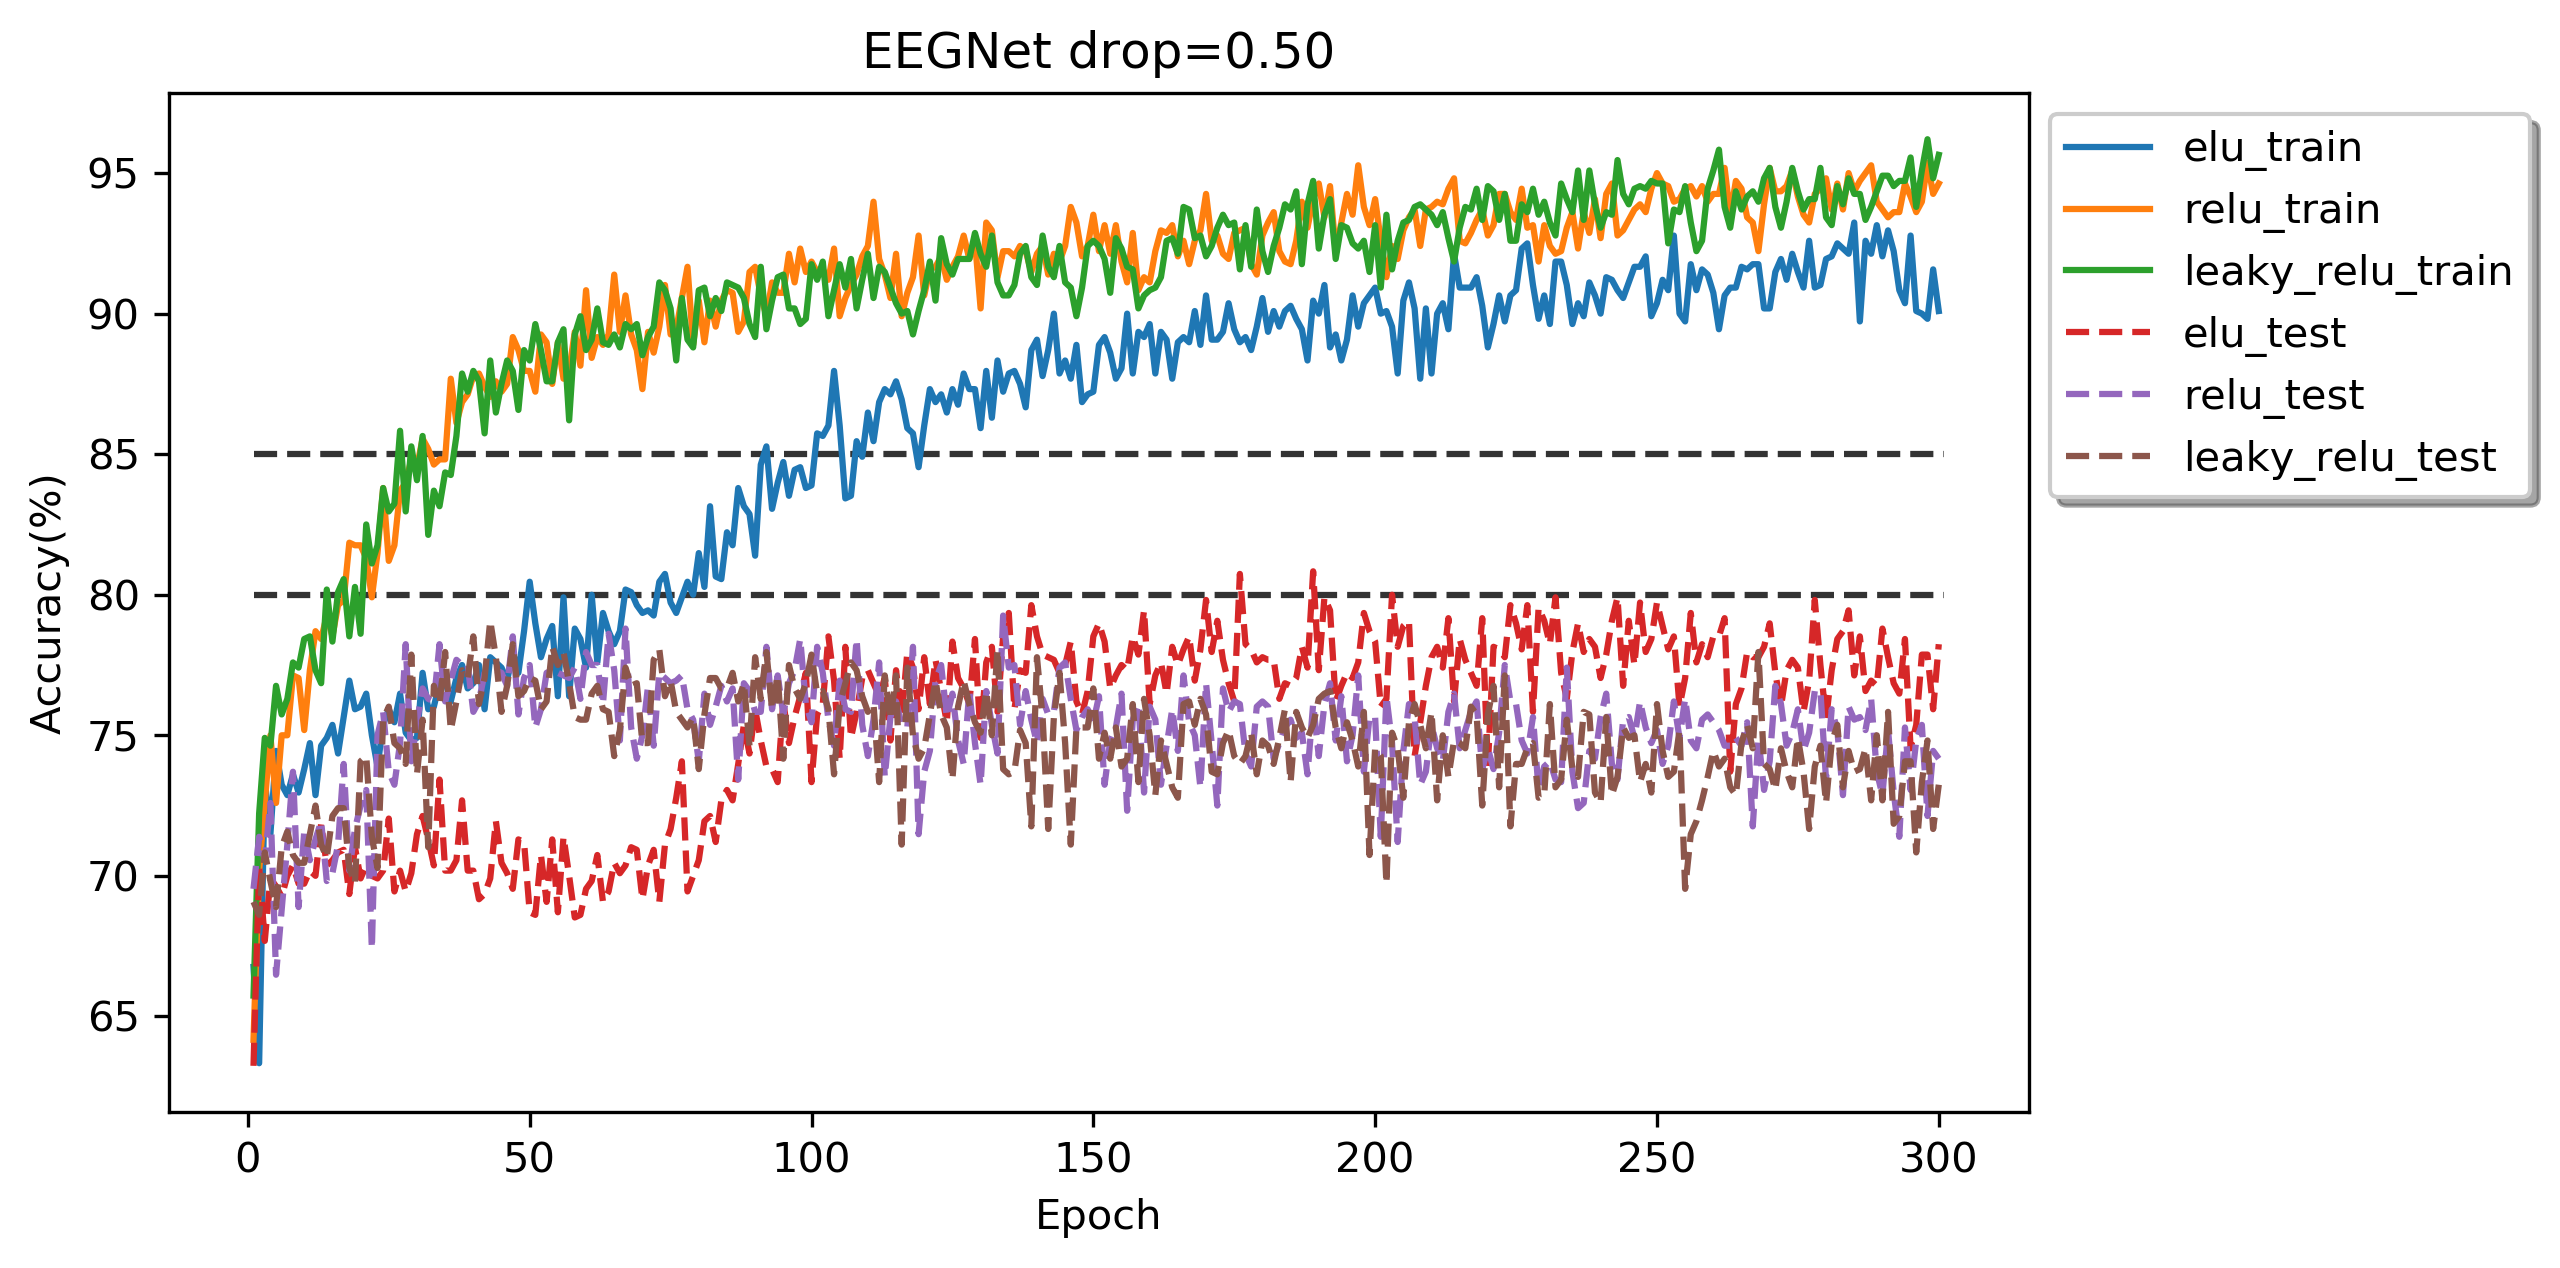
\includegraphics[width=\linewidth]{Images/EEGNetdrop=050.png}
\caption{EEGNet dropout rate = 0.5}
\end{figure}

\item dropout rate = 0.1

\begin{figure}[H]
\centering
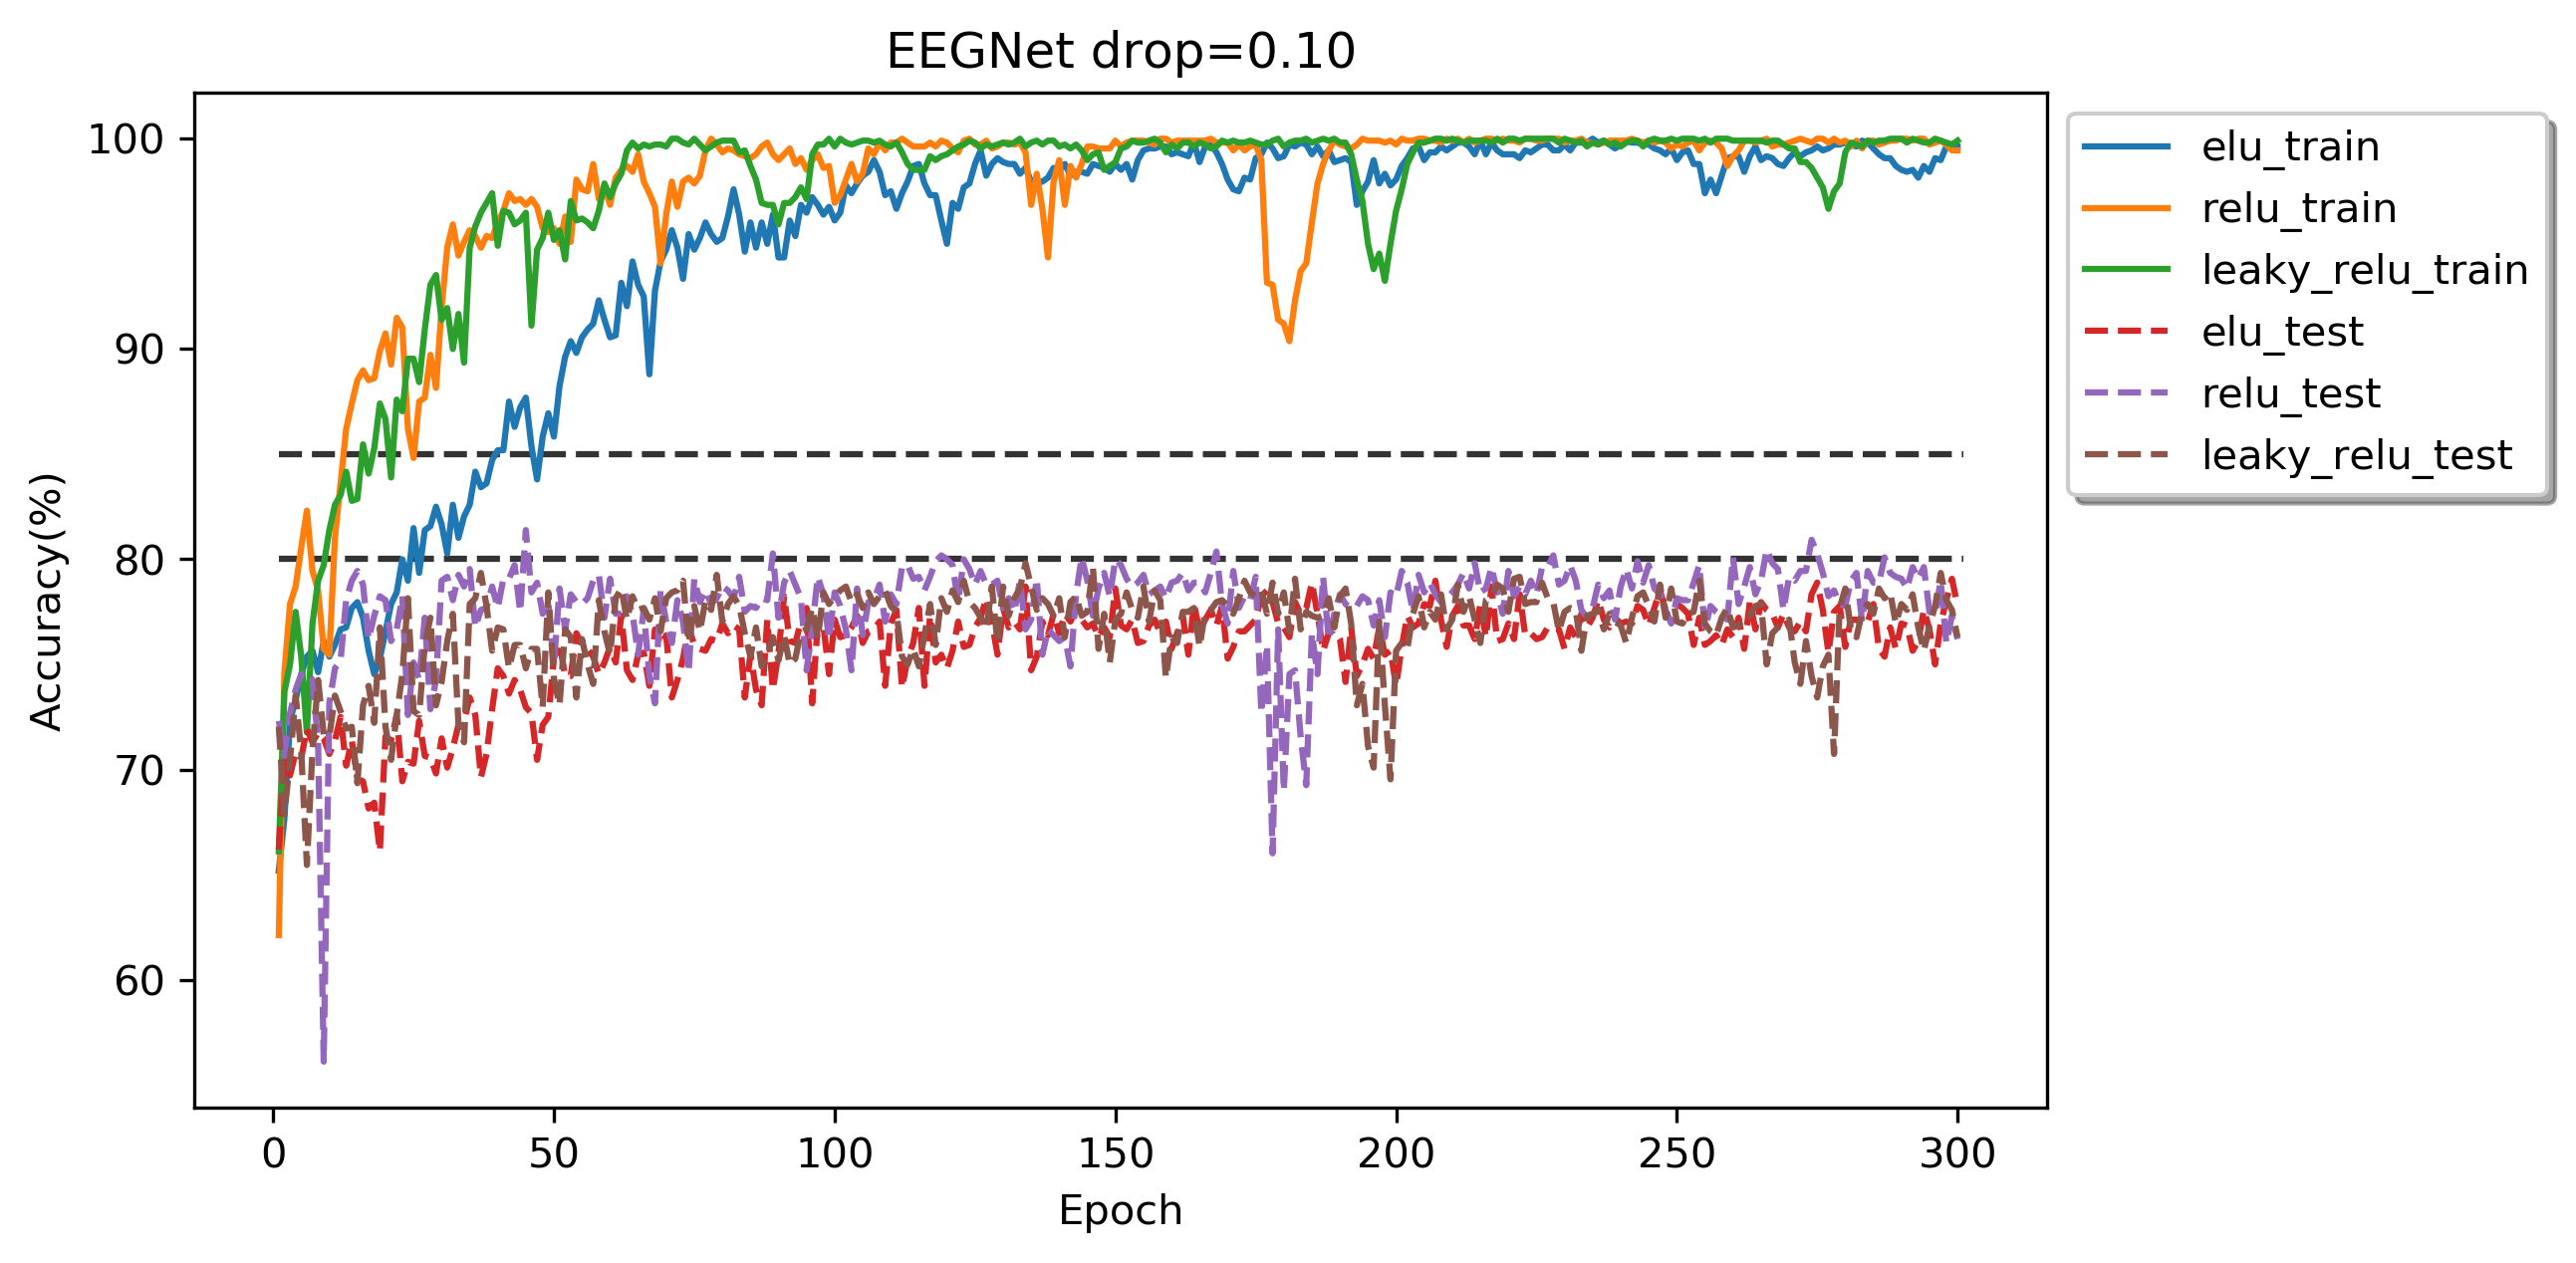
\includegraphics[width=\linewidth]{Images/EEGNetdrop=010.png}
\caption{EEGNet dropout rate = 0.1}
\end{figure}

\end{itemize}

When dropout rate is high, we can find training accuracy and distance between training and testing accuracy are low. So we need to trade-off dropout rate.

\end{document}